\structure{ИССЛЕДОВАТЕЛЬСКАЯ ЧАСТЬ}

\section{Обзор и анализ научной литературы в области обнаружения аномалий}

Развитие облачных инфраструктур и широкое распространение микросервисной архитектуры привели к массовому внедрению контейнеризации и систем оркестрации. В современных условиях платформа Kubernetes фактически стала промышленным стандартом для развёртывания, масштабирования и управления контейнеризованными приложениями. Вместе с такими преимуществами, как гибкость, масштабируемость и отказоустойчивость, использование Kubernetes сопровождается усложнением процессов обеспечения информационной безопасности. Это обусловлено высокой динамичностью среды, распределённым характером взаимодействия компонентов и большим количеством точек потенциального воздействия злоумышленника.

Традиционные средства защиты, включая сигнатурные системы обнаружения атак и правила контроля доступа, остаются важной частью системы обеспечения безопасности, однако в условиях постоянно изменяющегося поведения пользователей и сервисов их эффективность ограничена. Это стимулирует развитие подходов к обнаружению аномалий, основанных на методах машинного обучения и искусственного интеллекта, способных адаптироваться к изменяющимся условиям функционирования системы.

Сложность задачи обнаружения аномалий в контейнерных средах определяется многомерностью и разнородностью анализируемых данных. К таким данным относятся журналы аудита, метрики производительности, сетевой трафик и поведенческие характеристики контейнеров. Одновременно к системам обнаружения предъявляются строгие требования, связанные с вычислительными ограничениями, необходимостью работы в режиме, близком к реальному времени, и минимизацией числа ложных срабатываний. В работах, посвящённых безопасности контейнерных сред, выделяются ключевые механизмы обеспечения информационной безопасности, реализуемые в Kubernetes \cite{Container_Security_Extensive_Roadmap}. Эти механизмы охватывают различные уровни — от контроля доступа к API и управления правами до изоляции подов и защиты конфиденциальных данных. Однако даже их комплексное использование не гарантирует обнаружения ранее неизвестных атак и отклонений в поведении системы.

Целью систем обнаружения аномалий в Kubernetes-кластерах является выявление отклонений от нормального поведения, которые могут свидетельствовать о нарушениях политики безопасности, попытках несанкционированного доступа, злоупотреблении ресурсами или наличии вредоносной активности. Аномалии могут проявляться в виде нетипичных запросов к API, аномальных паттернов аутентификации, изменений сетевого взаимодействия между компонентами. Ручной анализ подобных событий затруднён из-за объёма и скорости поступления данных, что обуславливает необходимость применения автоматизированных методов анализа.

В существующих исследованиях и прикладных решениях можно выделить несколько основных подходов к обнаружению аномалий в контейнерных средах:

\begin{itemize}
    \item статические и правил-ориентированные методы, основанные на заранее заданных сигнатурах и эвристиках;
    \item методы, основанные на классических алгоритмах машинного обучения;
    \item методы, основанные на нейронных сетях и глубоком обучении.
\end{itemize}

Каждый из указанных подходов обладает своими преимуществами и ограничениями. Традиционные методы характеризуются высокой интерпретируемостью и низкими вычислительными затратами, однако плохо адаптируются к новым типам атак. Методы машинного обучения позволяют выявлять скрытые зависимости в данных, но требуют предварительной подготовки признаков и настройки моделей. Нейросетевые подходы, в свою очередь, демонстрируют высокую эффективность при анализе сложных и временных зависимостей, однако предъявляют повышенные требования к объёму данных и вычислительным ресурсам.

В рамках данного раздела будет проведён обзор и анализ научной литературы и прикладных исследований в области обнаружения аномалий в контейнерных средах. В частности, будут рассмотрены статические методы обнаружения аномалий, методы на основе классических алгоритмов машинного обучения, а также подходы, использующие нейронные сети. 

\subsection{Статические методы обнаружения аномалий}

Статические методы обнаружения аномалий являются одним из базовых подходов к обеспечению информационной безопасности и широко применяются в системах мониторинга и защиты информационных систем. Данные методы основываются на заранее заданных правилах, сигнатурах и эвристиках, определяющих допустимое поведение системы и выявляющих отклонения от него. В отличие от методов машинного обучения, статические подходы не требуют предварительного этапа обучения и функционируют на основе экспертных знаний о предметной области \cite{AD_Survey}.

В контейнерных средах, в частности в Kubernetes-кластерах, статические методы применяются для анализа audit-логов, сетевого взаимодействия, конфигурационных объектов и поведения пользователей и сервисных аккаунтов. Основной задачей является выявление заранее известных шаблонов аномального поведения, таких как попытки несанкционированного доступа, эскалации привилегий, использование запрещённых операций или отклонение от установленных политик безопасности.

К числу основных статических методов обнаружения аномалий относятся:

\begin{itemize}
    \item \textbf{Сигнатурный анализ (signature-based detection)} — основан на сопоставлении наблюдаемых событий с заранее известными шаблонами атак. Данный подход широко используется в системах обнаружения вторжений и позволяет эффективно выявлять известные угрозы с высокой точностью. Однако он не способен обнаруживать новые или модифицированные атаки \cite{Lightweight_Detection_Networks}.
    \item \textbf{Правило-ориентированные методы (rule-based detection)} — предполагают использование набора логических правил, описывающих допустимое и недопустимое поведение системы. В Kubernetes такие правила могут определять ограничения на использование привилегированных контейнеров, доступ к API или действия сервисных аккаунтов. Подобные механизмы в Kubernetes реализуются, например, с использованием Admission Controller \cite{KubernetesSecurityDocs}.
    \item \textbf{Пороговые методы (threshold-based detection)} — основаны на сравнении наблюдаемых метрик с заданными пороговыми значениями. Превышение допустимых уровней использования ресурсов (CPU, памяти) или частоты запросов может свидетельствовать о наличии аномалии. Простота реализации является преимуществом данного подхода, однако его эффективность зависит от корректности выбора порогов.
    \item \textbf{Методы белых и чёрных списков (whitelist/blacklist)} — предполагают явное задание разрешённых или запрещённых сущностей (пользователей, IP-адресов, операций). Отклонение от заданного списка интерпретируется как потенциальная аномалия. Данные методы часто применяются для контроля доступа и сетевого взаимодействия.
    \item \textbf{Методы, основанные на марковских процессах} — анализируют последовательности событий и вероятности переходов между состояниями системы.
\end{itemize}

\subsubsection{Сигнатурный анализ}

Сигнатурный анализ представляет собой метод, основанный на поиске совпадений между наблюдаемыми событиями и заранее известными шаблонами атак. Формально детектор можно представить как функцию:

$$
D(x) =
\begin{cases}
1, & \text{если } x \in S_{attack} \\
0, & \text{иначе}
\end{cases}
$$
где \(x\) — наблюдаемое событие; \\ \(S_{attack}\) — множество известных сигнатур атак \cite{IDS_survey_and_taxonomy}.

Данный подход широко применяется в системах IDS (Intrusion Detection Systems). Его основным преимуществом является высокая точность обнаружения известных атак и низкая вычислительная сложность. Однако он не способен выявлять ранее неизвестные угрозы.

\subsubsection{Правило-ориентированные методы}

Правило-ориентированные методы используют набор логических условий для описания допустимого поведения системы. Формально правило можно представить как предикат:

$$
R(x) = f(x_1, x_2, ..., x_n) \rightarrow \{0,1\},
$$
где \(x_i\) — признаки события; \\ \(f\) — логическая функция.

Инструменты для реализации такой логики (например, Falco \cite{falco}) реализуют сопоставление правил с событиями контейнеров и предоставляют как стандартный набор правил, так и механизм расширения этого набора пользовательскими правилами; аналогично, policy-ориентированные решения (Open Policy Agent \cite{opa}) применяют декларативные ограничения на этапе развертывания контейнера в кластере.

Преимущество правило-ориентированных методов состоит в их детерминированности и объяснимости. Однако та же детерминированность определяет и фундаментальное ограничение: правила не способно обнаружить ранее не встречавшиеся, тонкие или композиционные паттерны поведения (zero-day и эволюционирующие атаки), а также требуют постоянного ручного сопровождения - обновления и тестирования наборов правил по мере появления новых уязвимостей и изменчивости рабочих нагрузок.

\subsubsection{Пороговые методы}

Пороговые методы основаны на анализе статистических характеристик метрик системы. Пусть имеется наблюдаемая метрика \(x_t\), тогда аномалия определяется как:

$$
x_t \notin [\mu - k\sigma, \mu + k\sigma],
$$
где \(\mu\) — среднее значение; \\ \(\sigma\) — стандартное отклонение; \\ \(k\) — коэффициент чувствительности.

Также могут использоваться более сложные методы:
\begin{itemize}
    \item CUSUM (кумулятивные суммы);
    \item EWMA (экспоненциально взвешенное среднее);
\end{itemize}

Основное ограничение — чувствительность к изменению распределения данных и отсутствие учёта многомерных зависимостей.

\subsubsection{Методы и черных белых списков}

Метод белых списков основан на явном задании допустимых объектов:

$$
D(x) =
\begin{cases}
1, & x \in W \\
0, & x \notin W
\end{cases}
$$
где \(W\) — whitelist.

Метод черных списков, напротив, основан на запрете заранее известных нежелательных объектов:
\nopagebreak
$$
D(x) =
\begin{cases}
0, & x \in B \\
1, & x \notin B
\end{cases}
$$
где \(B\) — blacklist.

В Kubernetes такие методы применяются для контроля:

\begin{itemize}
    \item разрешённых/запрещенных IP-адресов;
    \item сервисных аккаунтов;
    \item допустимых образов контейнеров;
    \item фильтрации вредоносных сетевых запросов.
\end{itemize}

Недостатком является высокая статичность и необходимость регулярного обновления списков.

\subsubsection{Методы, основанные на марковских процессах}

Марковские методы рассматривают поведение системы как последовательность состояний \( S = \{s_1, s_2, \dots, s_n\} \), где переход между состояниями описывается условной вероятностью
$$
P(s_t \mid s_{t-1}).
$$

Таким образом, вероятность наблюдаемой последовательности состояний определяется как произведение вероятностей переходов:
$$
P(s_1, s_2, \dots, s_T) = \prod_{t=2}^{T} P(s_t \mid s_{t-1}).
$$

В задачах обнаружения аномалий модель обучается на нормальных последовательностях событий, формируя матрицу переходных вероятностей, отражающую типичное поведение системы. Если вероятность наблюдаемой последовательности оказывается ниже заданного порога, такая последовательность классифицируется как аномальная.

В контексте Kubernetes марковские модели применяются для анализа audit-логов, где состояния соответствуют типам API-запросов (например: \texttt{create}, \texttt{delete}, \texttt{patch}). Это позволяет выявлять нетипичные последовательности действий пользователей или сервисов. Основным преимуществом данного подхода является учёт временной структуры событий и зависимостей между последовательными действиями.

Однако ограничение классической марковской модели заключается в предположении о зависимости только от текущего состояния (свойство отсутствия памяти). Это снижает эффективность при анализе сложных атакующих сценариев, где важны долгосрочные зависимости и контекст.
\subsection{Алгоритмы машинного обучения}

Классические алгоритмы машинного обучения (МО) широко применяются для обнаружения аномалий в контейнерных средах благодаря способности выявлять скрытые закономерности в данных и определять отклонения от типичного поведения системы. В отличие от статических методов, такие алгоритмы опираются не на заранее заданные правила, а на статистические свойства обучающей выборки и особенности распределения наблюдений \cite{AD_Survey}.

Для анализа контейнерных сред и Kubernetes-кластеров классические алгоритмы МО могут применяться к различным типам данных: audit-логам, метрикам использования ресурсов, сетевой телеметрии, событиям взаимодействия между подами и признакам поведения пользователей или сервисных аккаунтов.

К числу наиболее распространённых алгоритмов машинного обучения, применяемых для обнаружения аномалий, относятся:

\begin{itemize}
    \item \textbf{K-ближайших соседей (K-Nearest Neighbors, K-NN)} — метод, основанный на оценке близости объекта к другим наблюдениям в пространстве признаков \cite{knn};
    \item \textbf{Isolation Forest (iForest)} — алгоритм, основанный на случайной изоляции объектов с помощью ансамбля деревьев \cite{iForest};
    \item \textbf{Random Cut Forest (RCF)} — метод, использующий ансамбль случайных разрезов пространства признаков и подходящий для потоковых данных \cite{RCF}.
\end{itemize}

\subsubsection{Метод K-ближайших соседей}

\textbf{K-NN} — алгоритм классификации и регрессии, основанный на гипотезе компактности, которая предполагает, что расположенные близко друг к другу объекты в пространстве признаков имеют схожие значения целевой переменной или принадлежат к одному классу \cite{knn}.

Принцип работы заключается в том, что для каждого нового наблюдения x алгоритм ищет k ближайших «соседей» в обучающей выборке и на основе расстояния/плотности соседей принимает решение (классификация) или вычисляет степень аномальности (anomaly score). Существуют несколько метрик расстояний:

\begin{itemize}
    \item Евклидово расстояние: \( d(\mathbf{x},\mathbf{y}) = \sqrt{\sum_{i=1}^n (x_i - y_i)^2} \);
    \item Манхэттен (L1) расстояние: \( d(\mathbf{x},\mathbf{y}) = \sum_{i=1}^n |x_i - y_i| \);
    \item Метрика Чебышева: \( d(\mathbf{x},\mathbf{y}) = \max_{i=1,\dots,n} |x_i - y_i| \).
\end{itemize}

Преимущества:

\begin{itemize}
    \item простота реализации: алгоритм легко адаптируется к разным типам данных;
    \item гибкость: может использоваться для задач классификации, регрессии и выявления аномалий;
\end{itemize}

Ограничения:

\begin{itemize}
    \item при большом объёме данных и высоком количестве признаков вычисление расстояний до всех соседей может быть ресурсоёмким;
    \item работает только с чиловыми признаками, поэтому необходима предобработка для данных. 
\end{itemize}

\subsubsection{Алгоритм Isolation Forest}

\textbf{Алгоритм Isolation Forest (iForest)} — метод обнаружения аномалий, основанный на идее изоляции объектов путём построения ансамбля случайных бинарных деревьев. Его фундаментальная концепция заключается в том, что образцы, которые проникают глубже в дерево, с меньшей вероятностью будут аномалиями, поскольку для их изоляции требуется больше разрезов, а образцы, которые оказываются в более коротких ветвях, указывают на аномалии, поскольку дереву проще отделить их от других наблюдений\cite{iForest}. 

На рисунке~\ref{fig:IF_png} показана концепция обнаружения аномалий с помощью Isolation Forest.

\begin{figure}
    \centering
    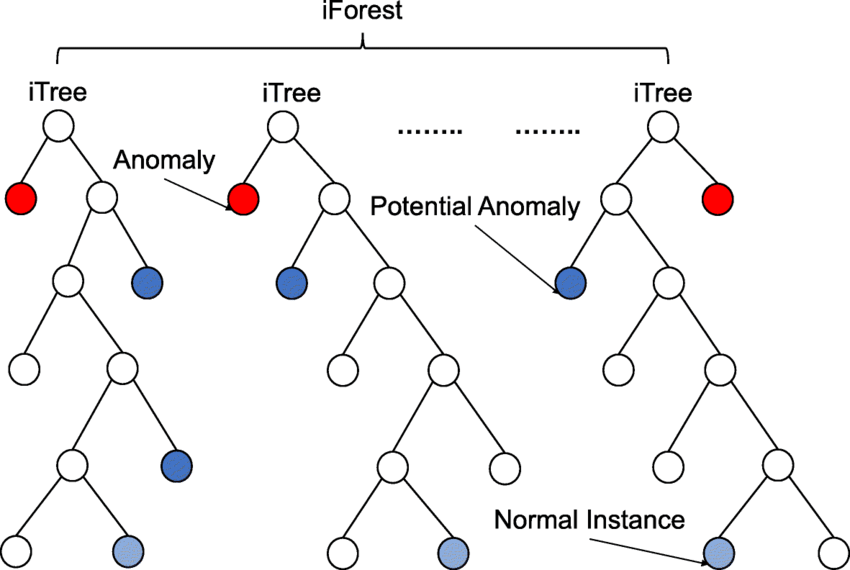
\includegraphics[scale=0.3]{inc/images/Isolation-Forest-learned}
    \caption{Схема выявления аномалий на основе Isolation Forest \cite{IF_png}.}
    \label{fig:IF_png}
\end{figure}

Принцип работы алгоритма заключается в следующем. Из исходного множества данных формируется ансамбль деревьев iTree \(t\), каждое из которых строится на случайно выбранной подвыборке данных размера \(\psi\). При построении дерева на каждом узле случайно выбирается признак \(q\) и случайный порог \(p\) из интервала \([\min_{x\in X} x_q,\;\max_{x\in X} x_q]\); затем пространство рекурсивно делится по этому порогу.

Построение iTree происходит следующем образом:

\begin{itemize}
    \item Выбирается подвыборка размера \(\psi\).
    \item Рекурсивно: пока \( |X|>1 \) и глубина ($height$) $<$ $height\_limit$:
    \begin{itemize}
        \item случайно выбрать признак \(q\) из множества признаков;
        \item случайно выбрать порог \(p\) из интервала $[\min_q,\;\max_q]$;
        \item разделить точки на множества $\{x\in X \mid x_q < p\}$ и $\{x\in X \mid x_q \ge p\}$ и рекурсивно строить дочерние узлы.
    \end{itemize}
    \item Остановить, если $|X|=1$ либо достигнут предельный уровень (height limit).
\end{itemize}

Для оценки аномальности объекта сначала вычисляют среднюю длину пути по всем деревьям ансамбля, \(E(h(x))\), приведенную в формуле~\ref{E_h}. 

\begin{equation}\label{E_h}
    E(h(x)) \;=\; \frac{1}{t}\sum_{i=1}^{t} h_i(x)
\end{equation}

где \(t\) — число деревьев.

Далее вычисляют нормирующую функцию \(c(n)\), используемую для приведения средней длины пути к масштабу, независимому от размера выборки \(n\), вычисляемую по формуле ~\ref{c_n}.

\begin{equation}\label{c_n}
    c(n) \;=\; 2H_{\,n-1} \;-\; \frac{2(n-1)}{n}
\end{equation}

где $H_{n}$ - гармоническое число

Наконец, для получения численной оценки аномальности применяют нормализацию средней длины пути \(E(h(x))\) по значению функции \(c(n)\); окончательная формула для вычисление значения аномальности приведена в ~\ref{s_x_n}.

\begin{equation}\label{s_x_n}
    s(x, n) \;=\; 2^{-\frac{E(h(x))}{c(n)}}
\end{equation}

Значение \(s(x,n)\), близкое к 1, указывает на высокую степень аномальности.

\subsubsection{Алгоритм Random Cut Forest}

\textbf{Алгоритм Random Cut Forest (RCF)} — это метод обнаружения аномалий, основанный на построении ансамбля случайных деревьев разрезов. В отличие от Isolation Forest, который изолирует точки с помощью последовательных случайных бинарных разбиений подвыборок, RCF формирует деревья непосредственно на основе случайных геометрических разрезов пространства признаков, что позволяет корректно обновлять и поддерживать модель при потоковом поступлении данных \cite{RCF}.

Основная идея заключается в том, что аномальные точки — это такие объекты, добавление или удаление которых вызывает значительное изменение геометрической структуры дерева, то есть существенно изменяет распределение разрезов, формирующих дерево. Алгоритм использует понятие размера проекции (displacement) и сопоставимой дисперсии (co-displacement), которые измеряют, насколько сильно добавление или удаление точки влияет на «геометрическую плотность» соседних точек в пространстве.

Алгоритм построения деревьев в RCF схож с алгоритмом iForest, за исключением того, как выбирается признак \(q\): вероятность выбора \(q\) пропорциональна длине стороны данного признака. Пусть имеется множество точек \(S = \{x_1, x_2, \dots, x_n\} \subset R^d\). Далее рекурсивно строится дерево \(T(S)\):
\begin{enumerate}
    \item Высчитываются длины сторон гиперпрямоугольника по формуле ~\ref{l_i}.

\begin{equation}\label{l_i}
    l_i \;=\; \max_{x \in S} x_i - \min_{x \in S} x_i
\end{equation}

    \item Строится гиперпрямоугольник (bounding box) $$B(S) = [\min_{x \in S} x_1, \max_{x \in S} x_1] \times  \dots \times [\min_{x \in S} x_d, \max_{x \in S} x_d],$$ охватывающий все точки множества \(S\).
    \item Вероятность выбора признака \(q \in Q\) высчитывается по формуле ~\ref{P_q}.  

\begin{equation}\label{P_q}
    P(q) \;=\; \frac{l_q}{\sum_{i \in Q} l_i}
\end{equation}

    \item Выбирается порог \(p\), равномерно выбранный из интервала \([\min_{x \in S} x_q, \max_{x \in S} x_q]\).
    \item Разрезом \((q,p)\) пространство \(B(S)\) разделяется на две части: $$S_L = \{ x\in S \mid x_q < p \}$$ и $$S_R = \{ x\in S \mid x_q \ge p \}$$
\end{enumerate}

В отличие от Isolation Forest, RCF не ограничивается метрикой глубины узла, а оценивает влияние объекта на геометрическую структуру данных. Это делает метод более устойчивым к изменениям плотности и эффективным для потоковых сценариев, где требуется онлайн-обновление модели без полной перестройки.
\subsection{Методы обнаружения аномалий на основе нейронных сетей}

Методы обнаружения аномалий на основе нейронных сетей в настоящее время являются одним из наиболее перспективных направлений анализа поведения информационных систем. Их основное преимущество заключается в способности автоматически извлекать скрытые закономерности из данных, учитывать нелинейные зависимости и моделировать сложные временные или структурные связи, которые трудно формализовать с помощью правил или классических алгоритмов машинного обучения.

К числу наиболее распространённых нейросетевых подходов к обнаружению аномалий относятся:

\begin{itemize}
    \item \textbf{Рекуррентные нейронные сети (Recurrent Neural Networks, RNN)} — используются для анализа последовательных данных и временных зависимостей;
    \item \textbf{Сети с долгой краткосрочной памятью (Long Short-Term Memory, LSTM)} — разновидность рекуррентных сетей, лучше сохраняющая долгосрочный контекст;
    \item \textbf{Автоэнкодеры (Autoencoders, AE)} — используются для моделирования нормального поведения и выявления аномалий по ошибке реконструкции.
\end{itemize}

\subsubsection{Рекуррентные нейронные сети (RNN)}

\textbf{Рекуррентные нейронные сети (RNN)} — это класс нейронных сетей, предназначенных для обработки последовательных данных с учётом временных зависимостей. RNN содержат рекуррентные связи, позволяющие скрытому состоянию на каждом временном шаге сохранять информацию о предыдущих входах. Это создаёт эффект памяти и контекста \cite{RNN}. Благодаря этому RNN подходят для задач, где важны порядок элементов и история наблюдений, например для прогнозирования временных рядов, анализа текста и речи \cite{RNNs_and_LSTMs}.

На рисунке~\ref{fig:RNN_arch} показана архитектура RNN. На каждом временном шаге $t$ входной вектор $x_t$ преобразуется с помощью матриц весов и функции активации в скрытое состояние $h_t$, которое затем используется для получения выхода $y_t$. Ключевое отличие RNN заключается в том, что при вычислении текущего состояния учитывается предыдущее скрытое состояние $h_{t-1}$, что и обеспечивает механизм памяти.

\begin{figure}
    \centering
    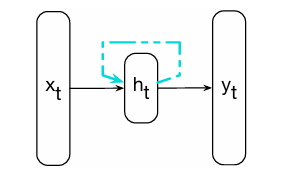
\includegraphics[scale=0.9]{inc/images/Simple-RNN-arch}
    \caption{Архитектура RNN \cite{RNNs_and_LSTMs}.}
    \label{fig:RNN_arch}
\end{figure}

RNN удобно представлять как сеть с прямой связью, «развернутую» по времени, где каждый узел скрытого слоя принимает на вход ранее вычисленное состояние. Такой подход показан на рисунке~\ref{fig:RNN_forward_inference}.

\begin{figure}
    \centering
    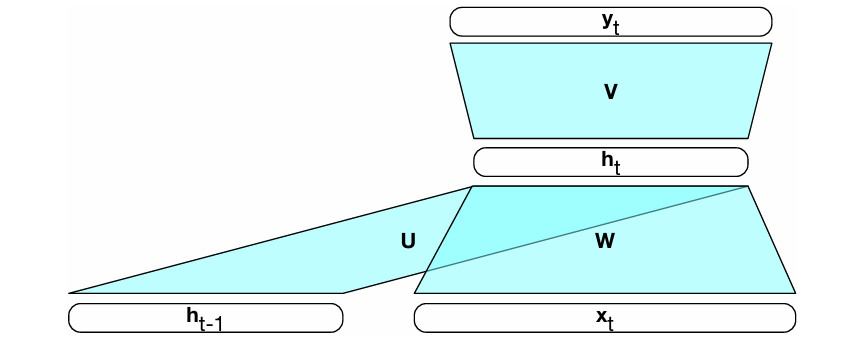
\includegraphics[scale=0.6]{inc/images/Simple-RNN-arch illustration feedforward}
    \caption{Архитектура RNN, представленная как сеть с прямой связью \cite{RNNs_and_LSTMs}.}
    \label{fig:RNN_forward_inference}
\end{figure}

Прямой проход RNN описывается следующими уравнениями. Скрытое состояние $h_t$ на шаге $t$ вычисляется по рекуррентному правилу, представленному в формуле~\ref{rnn_h_t}.

\begin{equation}\label{rnn_h_t}
    h_t = g(W x_t + U h_{t-1} + b_h),
\end{equation}

где $W$ — матрица весов для входа, $U$ — матрица рекуррентных весов, $b_h$ — вектор смещений, а $g(\cdot)$ — нелинейная функция активации, например $\tanh$ или ReLU. Выход сети \(y_t\) на шаге \(t\) определяется выражением, приведённым в формуле~\ref{rnn_y_t}.

\begin{equation}\label{rnn_y_t}
    y_t = f(V h_t + b_y),
\end{equation}

где $V$ — матрица весов между скрытым и выходным слоями, $b_y$ — вектор смещений выходного слоя, а $f(\cdot)$ — функция активации, часто используемая для нормализации выходов, например \texttt{softmax} для задач классификации.
Процедура вычисления выполняется последовательно по временным шагам: сначала $h_1$, затем $h_2$ и так далее до $h_T$. Таким образом, результат зависит от порядка элементов входной последовательности.

\textbf{Преимущества RNN:}
\begin{enumerate}
    \item Способность моделировать последовательные и временные зависимости между входными данными.
    \item Эффективное использование параметров: одни и те же веса применяются на всех временных шагах.
    \item Обработка входов переменной длины.
    \item Возможность онлайн-обучения на новых данных без полной перестройки модели.
\end{enumerate}

\textbf{Недостатки RNN:}
\begin{enumerate}
    \item Проблемы затухающих и взрывающих градиентов при обучении, затрудняющие захват долгосрочных зависимостей.
    \item Ограниченная способность к долгосрочной памяти в классических архитектурах.
    \item Последовательная природа вычислений затрудняет параллельное обучение и увеличивает вычислительную нагрузку.
\end{enumerate}

\subsubsection{Сети с долгой краткосрочной памятью (LSTM)}

\textbf{Long Short-Term Memory (LSTM)} — это разновидность рекуррентных нейронных сетей (RNN), разработанная для решения проблемы затухающих и взрывающих градиентов, характерной для классических RNN. Благодаря этому LSTM эффективно моделируют долгосрочные зависимости в последовательных данных, что сделало их одной из наиболее популярных архитектур для анализа временных рядов, текста и других последовательностей \cite{LSTM}.

Основная идея LSTM заключается в управлении потоком информации во времени с помощью механизмов ворот (gates). Ворота позволяют сети решать, какую информацию сохранить, обновить или забыть. Для этого в архитектуру LSTM добавляется вектор состояния ячейки (cell state), который играет роль долговременной памяти.

Каждый LSTM-блок содержит три основных типа ворот:

\begin{enumerate}
    \item \textbf{Ворота забывания (Forget gate)} — определяют, какая часть информации из предыдущего состояния $c_{t-1}$ должна быть сохранена или удалена;
    \item \textbf{Входные ворота (Input gate)} — контролируют добавление новой информации в состояние ячейки;
    \item \textbf{Выходные ворота (Output gate)} — определяют, какая часть обновлённого состояния $c_t$ передается в скрытое состояние $h_t$.
\end{enumerate}

\textbf{Ворота забывания} вычисляют взвешенную сумму скрытого слоя предыдущего состояния $h_{t-1}$ и текущего входного вектора $x_t$ и пропускают её через сигмоидную функцию (формула ~\ref{lstm_f_t}). Эта маска $f_t$ затем поэлементно умножается (произведение Адамара) на вектор предыдущего контекста $c_{t-1}$, чтобы удалить из него информацию, которая больше не требуется (формула ~\ref{lstm_k_t}).

\begin{equation}\label{lstm_f_t}
    f_t = \sigma(U_f h_{t-1} + W_f x_t)
\end{equation}

\begin{equation}\label{lstm_k_t}
    k_t = c_{t-1} \odot f_t
\end{equation}

\textbf{Входные ворота} управляют добавлением новой информации в память. Сначала вычисляется кандидат на обновление памяти $g_t$, представляющий возможное новое содержимое контекста (формула~\ref{lstm_g_t}).

\begin{equation}\label{lstm_g_t}
    g_t = \tanh(U_g h_{t-1} + W_g x_t)
\end{equation}

Функция $\tanh(\cdot)$ ограничивает значения в диапазоне $(-1, 1)$, что повышает устойчивость обновлений. Далее вычисляется сигмоидная маска $i_t$, определяющая степень добавления новых данных в память (формула~\ref{lstm_i_t}).

\begin{equation}\label{lstm_i_t}
    i_t = \sigma(U_i h_{t-1} + W_i x_t)
\end{equation}

Эти два вектора поэлементно умножается (формула~\ref{lstm_j_t}), что формирует итоговое обновление памяти.

\begin{equation}\label{lstm_j_t}
    j_t = g_t \odot i_t
\end{equation}

Итоговое состояние ячейки вычисляется как сумма модифицированного старого состояния $k_t$ и нового добавления $j_t$ (формула~\ref{lstm_c_t}).

\begin{equation}\label{lstm_c_t}
    c_t = k_t + j_t
\end{equation}

\textbf{Выходные ворота} определяют, какая часть обновлённого контекста $c_t$ используется для формирования скрытого состояния $h_t$. Сначала вычисляется маска выхода $o_t$ (формула~\ref{lstm_o_t}).

\begin{equation}\label{lstm_o_t}
    o_t = \sigma(U_o h_{t-1} + W_o x_t)
\end{equation}

Затем скрытое состояние определяется как поэлементное произведение маски выхода $o_t$ и нелинейно преобразованного контекста (формула~\ref{lstm_h_t}).

\begin{equation}\label{lstm_h_t}
    h_t = o_t \odot \tanh(c_t)
\end{equation}

Рисунок~\ref{fig:LSTM_arch} иллюстрирует полный процесс вычислений в одном блоке LSTM. Блок принимает на вход текущее наблюдение, скрытое состояние предыдущего шага и состояние ячейки, после чего формирует обновлённые значения на выходе. Именно скрытое состояние $h_t$ используется как выход LSTM на каждом временном шаге.

\begin{figure}
    \centering
    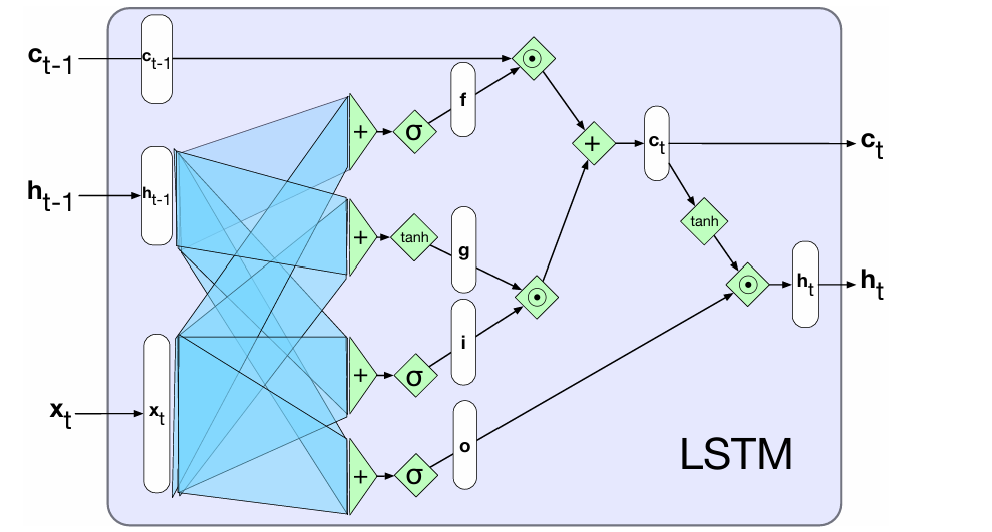
\includegraphics[scale=0.8]{inc/images/LSTM-arch}
    \caption{Архитектура LSTM \cite{RNNs_and_LSTMs}.}
    \label{fig:LSTM_arch}
\end{figure}

Архитектура LSTM естественным образом подходит для анализа метрик и логов Kubernetes-кластера, поскольку она оптимизирована для работы с последовательными и временными рядами.

\subsubsection{Автоэнкодеры}

\textbf{Автокодировщик (Autoencoder, AE)} — это нейросетевая модель, которая обучается сжимать входные данные в компактное латентное представление и восстанавливать исходные данные по этому представлению. Цель обучения состоит в минимизации ошибки восстановления, например MSE или бинарной кросс-энтропии, благодаря чему модель извлекает информативные признаки входных данных \cite{AE}.

Архитектура автокодировщика состоит из двух основных частей:

\begin{itemize}
    \item \textbf{Encoder} — преобразует входной вектор признаков $x$ в компактное скрытое представление $z$;
    \item \textbf{Decoder} — восстанавливает исходный вектор $\tilde{x}$ по скрытому представлению $z$.
\end{itemize}

На рисунке~\ref{fig:AE_arch} представлена типичная архитектура автокодировщика. Входной вектор признаков проходит через несколько полносвязных слоёв Encoder, которые последовательно уменьшают размерность представления. Центральный слой формирует латентное пространство, содержащее компактное описание входных данных. Затем Decoder восстанавливает исходный вектор признаков.

\begin{figure}
    \centering
    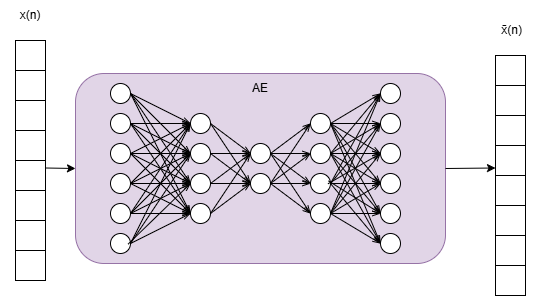
\includegraphics[scale=0.6]{inc/images/autoencoder_architecture}
    \caption{Архитектура классического Autoencoder.}
    \label{fig:AE_arch}
\end{figure}

Математически процесс кодирования описывается в формуле~\ref{eq:encoder}.

\begin{equation}\label{eq:encoder}
    z = g(W_e x + b_e)
\end{equation}

где $W_e$ — матрица весов Encoder, $b_e$ — вектор смещений, а $g(\cdot)$ — функция активации.

Процесс декодирования, описанный в формуле~\ref{eq:decoder}, восстанавливает исходный вектор признаков.

\begin{equation}\label{eq:decoder}
    \tilde{x} = f(W_d z + b_d)
\end{equation}

где $W_d$ — матрица весов Decoder, $b_d$ — вектор смещений, а $f(\cdot)$ — функция активации выходного слоя.

Таким образом, автокодировщик аппроксимирует функцию восстановления, представленную в формуле~\ref{eq:ae_mapping}.

\begin{equation}\label{eq:ae_mapping}
    \tilde{x} = f(W_d g(W_e x + b_e) + b_d)
\end{equation}